\documentclass[../cheatSheetAlgoritmi.tex]{subfiles}
\begin{document}

\section{Esami anni passati}
\subsection{Esame 07/02/2019}
\textbf{Esercizio A1} Trovare un limite superiore, il più stretto possibile per la seguente equazione di ricorrenza: \
\begin{equation*}
  	T(n)=\begin{cases}
    	T(\lfloor n/2 \rfloor) + T(\lfloor n/4 \rfloor)+ T(\lfloor n/8 \rfloor)+ 2T(\lfloor n/16 \rfloor) + 1 & \text{$n > 16$}\\
    	1 & \text{$n \leq 16$}
  	\end{cases}
\end{equation*} \\
\textbf{Soluzione A1} Non possiamo applicare il master theorem quindi proviamo a risolvere il problema per tentativi. Proviamo con il metodo di sostituzione a verificare e vale T(n) = $\mathcal{O}(n)$. Dimostriamo per induzione.\
\begin{itemize}
	\item Ipotesi induttiva: T(k) $\leq$ ck, per k $<$ n
	\item Passo induttivo:
\begin{equation*}
\begin{aligned}	
T(n)= T(\lfloor n/2 \rfloor) + T(\lfloor n/4 \rfloor)+ T(\lfloor n/8 \rfloor)+ 2T(\lfloor n/16 \rfloor) + 1\\
\text{$\leq$} c\lfloor n/2 \rfloor + c\lfloor n/4 \rfloor+ c\lfloor n/8 \rfloor+ 2c\lfloor n/16 \rfloor + 1\\ 
\text{$\leq$}  \dfrac{1}{2}cn + \dfrac{1}{4}cn + \dfrac{1}{8}cn + \dfrac{1}{8}cn + 1\\
=  cn + 1 \text{$\leq$} cn \\
\end{aligned}
\end{equation*}
L'ultima disequazione è falsa per un termine di ordine inferiore. 
\end{itemize}

Proviamo a dimostrare che 
\begin{equation*}
  \exists b \text{$>$} 0, \exists c \text{$>$} 0, \exists m \text{$\geq$} 0, : T(n) \text{$\leq$} cn-b, \forall n \text{$\geq$} m
\end{equation*}
\begin{itemize}
	\item Ipotesi induttiva: T(k) $\leq$ ck-b, per k $<$ n
	\item Passo induttivo:
	\begin{equation*}
		\begin{aligned}	
			T(n)= T(\lfloor n/2 \rfloor) + T(\lfloor n/4 \rfloor)+ T(\lfloor n/8 \rfloor)+ 2T(\lfloor n/16 \rfloor) + 1\\
			\text{$\leq$} c(lfloor n/2 \rfloor -b + c\lfloor n/4 \rfloor -b+ c\lfloor n/8 \rfloor -b + 2(c \lfloor n/16 \rfloor -b) + 1\\ 
			\text{$\leq$}  \dfrac{1}{2}cn -b + \dfrac{1}{4}cn -b + \dfrac{1}{8}cn -b + \dfrac{2}{16}cn -2b + 1\\
=  cn -5b + 1 \text{$\leq$} cn -b \\
		\end{aligned}
	\end{equation*}
	L'ultima disequazione è vera per ogni c e per b $\geq$ $\dfrac{1}{4}$. 
	\item Caso base: T(n)=1 $\leq$ cn-b, per tutti i valori di n compresi tra 1 e 16, ovvero: 
	\begin{equation*}
		c \text{$\geq$} \dfrac{b+1}{n}, \forall n: 	\text{$1 \leq n \leq 16$}
	\end{equation*}
	I valori $\dfrac{b+1}{n}$ sono minori o uguali di 5/4 (per T(1) vale 5/4), per 1 $\leq$ n $\leq$ 16; quindi tutte queste disequazioni sono soddisfatte da c $geq$ 5/4. 
\end{itemize}
Abbiamo quindi dimostrato che T(n)= $\mathcal{O}(n)$, con m= 1 e c $\geq$ 5/4.
\newpage 
\textbf{Le croci}  \\
Si consideri una matrice binaria $M$ di dimensione $n \times n$. Scrivere un algoritmo
\begin{center}
\textbf{int} cross(\textbf{int}[ ][ ] M,\textbf{int} n)
\end{center}
che restituisca la dimensione della più grande croce composta da valori $1$ presente nella matrice. Una croce è compostada un bit $1$ centrale e quattro braccia di uguale lunghezza,contenenti bit $1$. Non deve essere necessariamente circondata da bit $0$. \\
Per esempio, la croce visibile nell’esempio è composta da 17 valori 1e l’algoritmo dovrà restituire 17.
\begin{center}
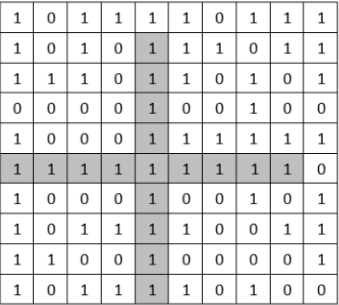
\includegraphics{ ../img/esame_07022019}
\end{center}
\textbf{Soluzione} \\
Il docente propone un approccio basato su programmazione dinamica per risolvere il seguente problema. \\ Si costruiscono quattro matrici di appoggio, chiamate $L,R,U,D$ (left, right, up,down). \\
Le caselle $L[i][j]$, $R[i][j]$, $U[i][j]$, $D[i][j]$ contiene la più lunga fila di valori $1$ che si estende a partire dalla cella $(i, j)$(compresa) nella direzione sinistra, destra, alto, basso. \\
Tali vettori vengono calcolati come segue: 
\begin{equation*}
  	L[i][j] =\begin{cases}
    	M[i][j] & \text{$j = 1$}\\
    	L[i][j-1] + 1 & \text{$j > 1$ \textbf{and} $M[i][j] = 1$}\\
    	0 & \text{$j > 1$ \textbf{and} $M[i][j] = 0$}
  	\end{cases}
\end{equation*}
\begin{equation*}
  	R[i][j] =\begin{cases}
    	M[i][j] & \text{$j = n$}\\
    	R[i][j+1] + 1 & \text{$j < n$ \textbf{and} $M[i][j] = 1$}\\
    	0 & \text{$j < n$ \textbf{and} $M[i][j] = 0$}
  	\end{cases}
\end{equation*}
\begin{equation*}
  	D[i][j] =\begin{cases}
    	M[i][j] & \text{$i = 1$}\\
    	D[i+1][j] + 1 & \text{$i < n$ \textbf{and} $M[i][j] = 1$}\\
    	0 & \text{$i < n$ \textbf{and} $M[i][j] = 0$}
  	\end{cases}
\end{equation*}
\begin{equation*}
  	U[i][j] =\begin{cases}
    	M[i][j] & \text{$i = 1$}\\
    	U[i-1][j] + 1 & \text{$i > 1$ \textbf{and} $M[i][j] = 1$}\\
    	0 & \text{$i > 1$ \textbf{and} $M[i][j] = 0$}
  	\end{cases}
\end{equation*}
Ovvero partendo dalla posizione $(i, j)$ si considerano le somme di 1 sulla rispettiva dimensione, nella cella considerata precedentemente, solo se il valore sulla matrice originale $M$ è 1. \\
Una volta calcolati questi valori è possibile trovare la più grande croce il cui centro è collocato in $(i, j)$ semplicemente calcolando: 
\begin{center}
$min(L[i][j], R[i][j], U[i][j], D[i][j]) \cdot 4 - 3$
\end{center}
Ovvero si usa la più lunga sequenza di valori $1$ consecutiva nelle quattro direzioni possibili e si usa il minimo di questi valori in quanto limita la dimensione della nostra croce. A questo punto, ora che conosciamo il lato della croce più grande possibile centrata in $(i, j)$, calcoliamo in numero di celle che la compongono moltiplicando la dimensione del braccio per 4 e sottraendo 3. Si sottrae 3 dato che in tutte definizioni di $L[i][j], R[i][j], U[i][j]$ e $D[i][j]$ la cella (i, j) è compresa, ed è necessario considerarla una singola volta.
\begin{lstlisting}[ caption = Croce massimale formata da sequenze di 1]
int cross(int[][] M, int n)
	int[][] L = new int[1...n][1...n]
	int[][] R = new int[1...n][1...n]
	int[][] U = new int[1...n][1...n]
	int[][] D = new int[1...n][1...n]
	for j = 1 to n do
		U[1][j] = M[1][j]
		D[n][j] = M[n][j]
	for i = 1 to n do
		L[i][1] = M[i][1]
		R[i][n] = M[i][n]
	for i = 2 to n do
		for j = 2 to n do
			L[i][j] = iif(M[i][j] $==$ 0, 0, L[i][j-1] + 1)
			U[i][j] = iif(M[i][j] $==$ 0, 0, U[i-1][j] + 1)
	for i = n - 1 downto 1 do
		for j = n - 1 downto 1 do
			R[i][j] = iif(M[i][j] $==$ 0, 0, R[i][j+1] + 1)
			D[i][j] = iif(M[i][j] $==$ 0, 0, D[i+1][j] + 1)
	int maxSoFar = 0
	for i = 1 to n do
		for j = 1 to n do
			int size = min(L[i][j], R[i][j], U[i][j], D[i][j]) $\cdot$ 4 - 3
			maxSoFar = max(maxSoFar, size)
	return maxSoFar
\end{lstlisting}
Come è facilmente intuibile, il costo computazionale di tale procedura è di $\Theta(n^2)$.
\newpage
\end{document}